\section{MANO Benchmarking Framework} 

\subsection{Introduction}

MANO Benchmarking Framework (MBF) is a result of a small script that was used to run the experiments discussed in the previous sections. The idea of MBF is to provide MANO developers with a generic framework for running experiments on MANO. MBF mainly provides the following 1) Easy interfacing with MANO instances by using python-mano-wrappers, 2) Ability to run experiments with different service descriptors, 3) Collection of performance metrics in convenient data format and 4) Flexible graphing mechanism of the collected data. 

\subsection{Design}

MBF is designed for ease of use and low barrier to entry for developers. We explain the choice of tools that are used in MBF in the following list.

\begin{itemize}
	\item{\textbf{Netdata\footnote{https://github.com/netdata/netdata}}} is the metrics monitoring system for MBF. Netdata captures relevant system metrics and provide powerful APIs to query the recorded data in a suitable format.
	\item{\textbf{Python}} as the choice of scripting language was obvious as the MANOs itself are implemented in python.
	\item{\textbf{python-mano-wrappers}} is used to provide access to REST APIs of MANOs from python.
	\item{\textbf{Docker}} is used to containerize MBF, thus making it easy to distribute and portable.
	\item{\textbf{Matplotlib}} is the graphing library for MBF due to its flexibility and ease of use.
	\item{\textbf{Flask}} as a small python server that can be used to provide additional interactions with the experiment runner.

\end{itemize}

 

\subsection{Parameters and KPIs} 
\todo[inline]{Explain the variable parameters and possible KPIs from the experiments}

\subsection{Steps for the automated experiment run} 
\todo[inline]{A walkthrough of the experiment runner}

\subsection{Example Use Cases}
\todo[inline]{Explain results acquired from MANO benchmarking tool}

\subsubsection{Comparison of different network services} 

Comparison of different network services

\begin{figure}[h]
	\centering
	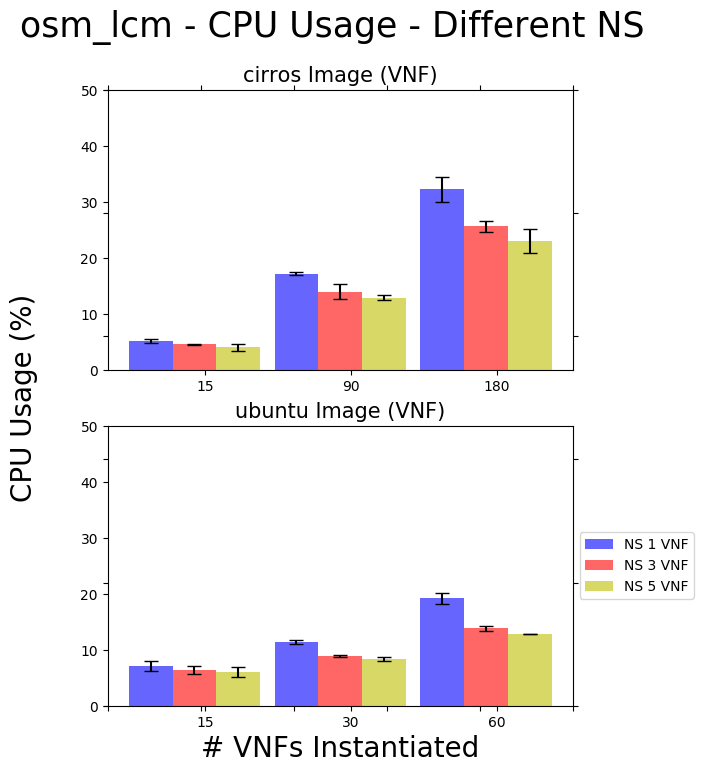
\includegraphics[width=0.7\linewidth]{figures/scalability_graphs/Docker-Grouped-Cases/osm/osm_lcm-Mean-CPU-Cases}
	\caption{}
	\label{fig:osmlcm-mean-cpu-cases}
\end{figure}

\begin{figure}[h]
	\centering
	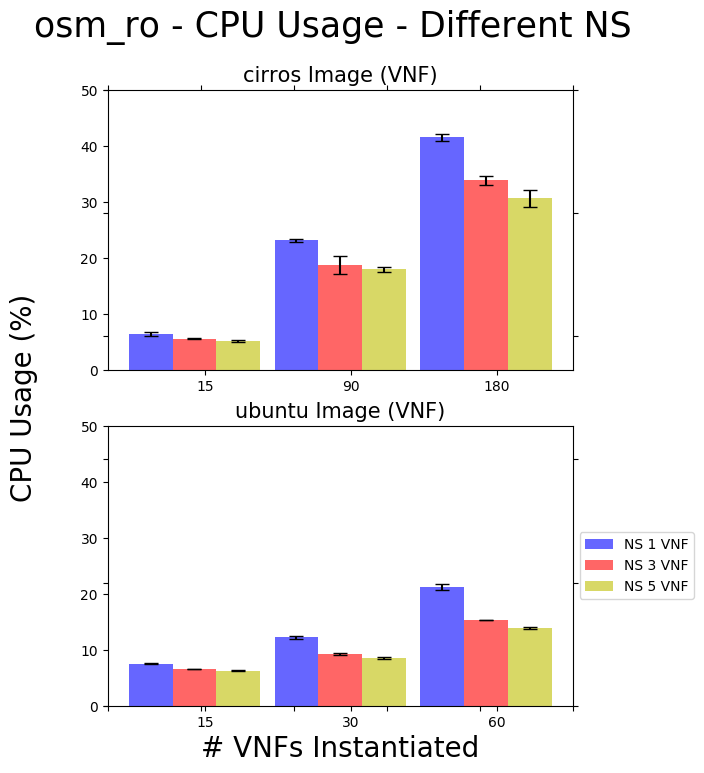
\includegraphics[width=0.7\linewidth]{figures/scalability_graphs/Docker-Grouped-Cases/osm/osm_ro-Mean-CPU-Cases}
	\caption{}
	\label{fig:osmro-mean-cpu-cases}
\end{figure}


\subsubsection{Container vs VM Orchestration} 

Container vs VM Orchestration

\begin{figure}[h]
	\centering
	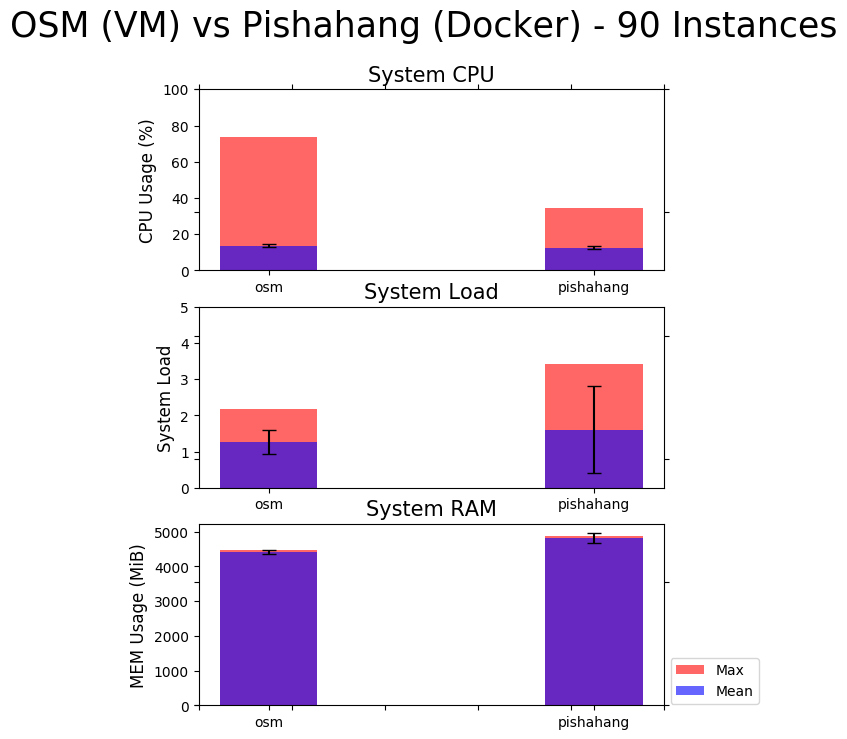
\includegraphics[width=0.7\linewidth]{figures/scalability_graphs/Comparison-VM-Docker/System_metrics_comparison}
	\caption{}
	\label{fig:systemmetricscomparison}
\end{figure}

\begin{figure}[h]
	\centering
	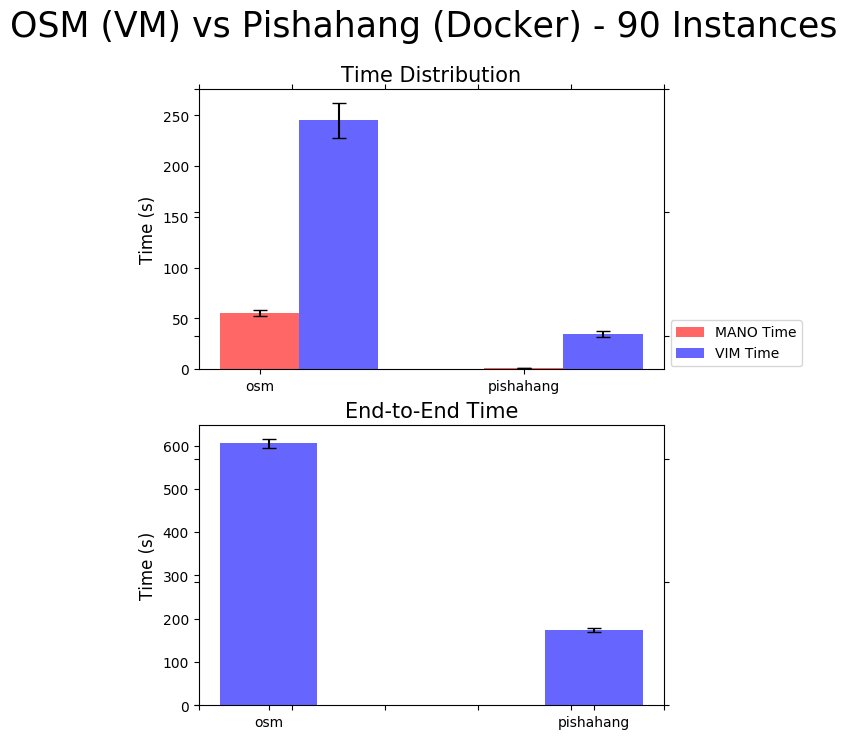
\includegraphics[width=0.7\linewidth]{figures/scalability_graphs/Comparison-VM-Docker/Time_comparison}
	\caption{}
	\label{fig:timecomparison}
\end{figure}


\subsubsection{Scaling Plugin Evaluation}

\begin{figure}[h]
	\centering
	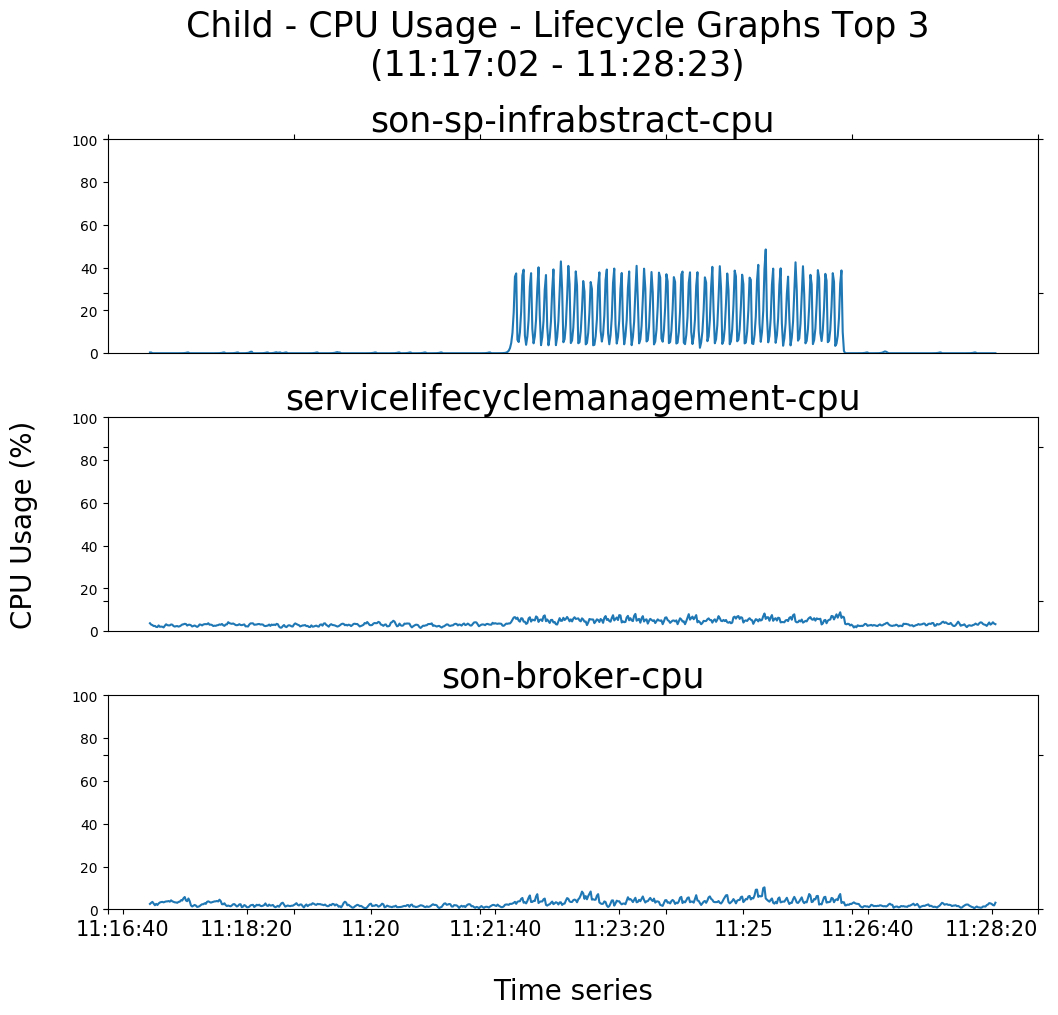
\includegraphics[width=0.7\linewidth]{figures/scalability_graphs/Scalability-Evaluation/Child-TOP-3-Lifecycle}
	\caption{Child scaling}
	\label{fig:child-top-3-lifecycle}
\end{figure}

\begin{figure}[h]
	\centering
	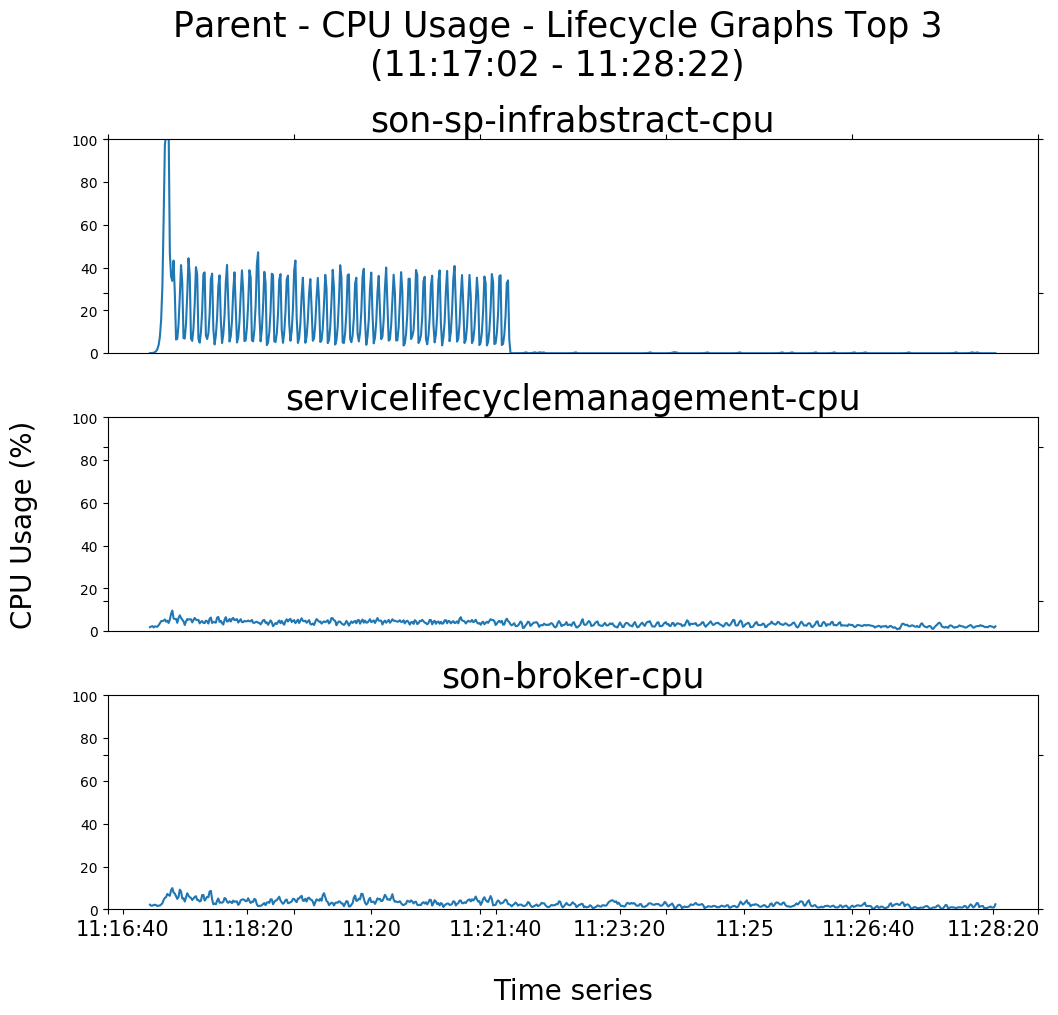
\includegraphics[width=0.7\linewidth]{figures/scalability_graphs/Scalability-Evaluation/Parent-TOP-3-Lifecycle}
	\caption{Parent Scaling}
	\label{fig:parent-top-3-lifecycle}
\end{figure}


\subsection{Future scope}